\subsection{Experiment 8: Unregularized and Removal of Elastic Net} \label{sec:exp8}

In Experiment 5, a bug was identified and the author had to eliminate the elastic net implementation, which necessitated a complete rewrite of the models and training loop. Due to this, no regularization was enforced in this experiment.

However, aside from the absence of regularization and elastic net, the experimental setup is identical to the larger test performed in Experiment 7, which featured a model containing roughly 50 million parameters.

In epoch 37, the experiment incurred a total loss of $1.832$, consisting of the generator loss of $0.693$ and the discriminator loss of $1.139$.

Training of the model resulted in a sudden collapse at epoch 37, with inexplicable loss values plummeting to as low as 0 thereafter.

To gain insight into the training progress, two spectrograms were generated: one for epoch 37 (see Figure~\ref{fig:exp8_37_results}) and another for epoch 49, which marked the end of training (see Figure~\ref{fig:exp8_results}).

Additionally, a histogram depicting the values present in the generated encodings has been included in this experiment.

\begin{figure}[!ht]
    \centering
    \begin{subfigure}{0.4\textwidth}
        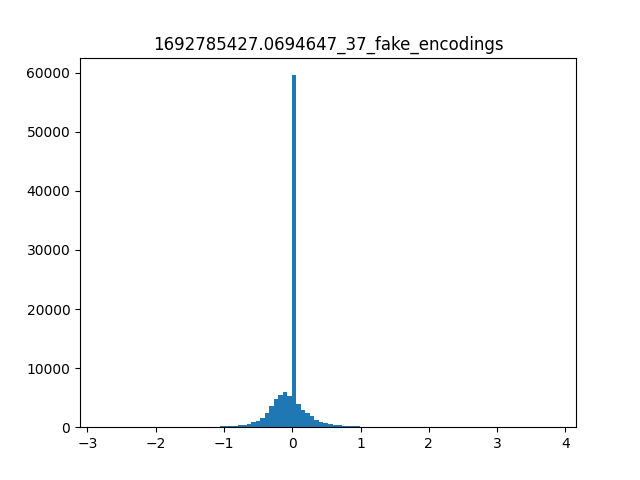
\includegraphics[width=\textwidth]{figures/4.5-results/exp8_37_hist.png}
        \caption{Histogram of the generated embeddings for Experiment 8 in epoch 37.}
        \label{fig:exp8_37_hist}
    \end{subfigure}
    \begin{subfigure}{0.4\textwidth}
        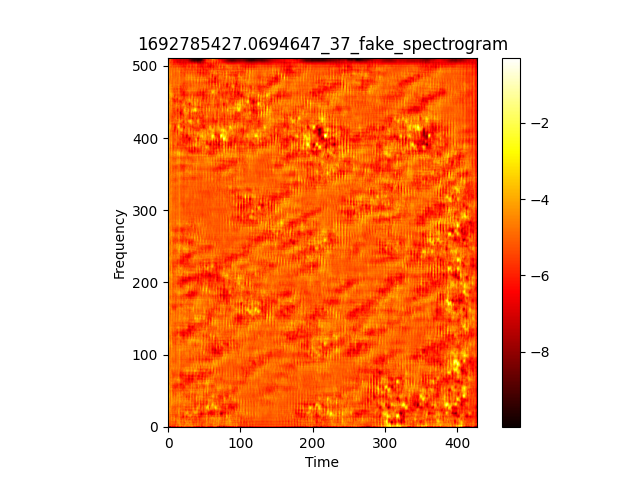
\includegraphics[width=\textwidth]{figures/4.5-results/exp8_37_spectrogram.png}
        \caption{Spectrogram generated in Experiment 8 in epoch 37.}
        \label{fig:exp8_37_spectrogram}
    \end{subfigure}
    \caption{Results of Experiment 8 in epoch 37.}
    \label{fig:exp8_37_results}
\end{figure}

\begin{figure}[!ht]
    \centering
    \begin{subfigure}{0.3\textwidth}
        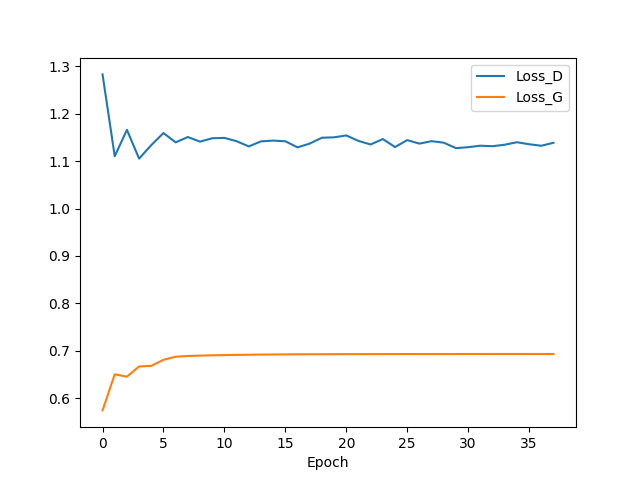
\includegraphics[width=\textwidth]{figures/4.5-results/exp8_loss.png}
        \caption{Evolving losses throughout the training process for Experiment 8.}
        \label{fig:exp8_loss}
    \end{subfigure}
    \begin{subfigure}{0.3\textwidth}
        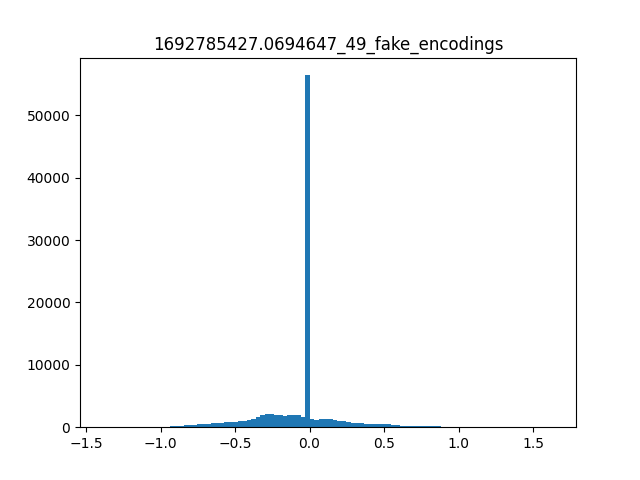
\includegraphics[width=\textwidth]{figures/4.5-results/exp8_hist.png}
        \caption{Histogram of the generated embeddings for Experiment 8.}
        \label{fig:exp8_hist}
    \end{subfigure}
    \begin{subfigure}{0.3\textwidth}
        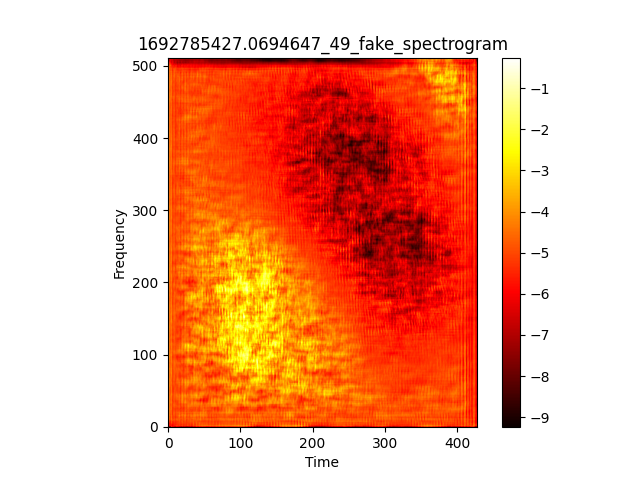
\includegraphics[width=\textwidth]{figures/4.5-results/exp8_spectrogram.png}
        \caption{Spectrogram generated in Experiment 8.}
        \label{fig:exp8_spectrogram}
    \end{subfigure}
    \caption{Results of Experiment 8 at the end of training.}
    \label{fig:exp8_results}
\end{figure}